\documentclass["../Cours.tex"]{subfiles}

\begin{document}
\chapitre{Équation}

\partie{Concept}

\definition{Une équation est une égalité contenant une variable \emph{inconnue} désignée par une lettre.\\ Les nombres pour lesquels l'égalité est vraie sont les solutions de l'équation.}

\begin{listedexemples}
    \item $2x+5=3$\\ 
    Est-ce que 4 est solution de l'équation ?\\$2 \times 4 + 5 = 13 \neq 3$
    \item $7x+5 = 6x+6$\\ 
    Est-ce que 0 est solution de l'équation ?\\
    \begin{align*}
        7 \times 0 + 5 = 5 & ~~\mbox{(membre de gauche)}\\
        6 \times 0 + 6 = 6 & ~~\mbox{(membre de droite)}
    \end{align*}
    Est-ce que 1 est solution de l'équation ?\\
    \begin{align*}
        7 \times 1 + 5 = 12 & ~~\mbox{(membre de gauche)}\\
        6 \times 1 + 6 = 12 & ~~\mbox{(membre de droite)}
    \end{align*}
    Donc 1 est solution de l'équation. On va noter $S = \left\{ 1 \right\}$.
\end{listedexemples}

\partie{Résolution d'équations du premier degré}

\paragraphe{rouge}{Règle 1}{Dans une équation, on peut ajouter ou retirer la même quantité dans chaque membre de l'équation.}

\exemple{
\begin{align*}
    7x + 5 &= 12 \\
    7x + 5 \textcolor{rouge}{+10} &= 12 \textcolor{rouge}{+10} & \mbox{(on ajoute 10 de chaque côté)}\\ 
    7x + 5 \textcolor{rouge}{-2x} &= 12 \textcolor{rouge}{-2x} & \mbox{(on enlève 2x de chaque côté)}\\ 
\end{align*}
}

\paragraphe{rouge}{Règle 2}{Dans une équation, on peut multiplier ou diviser chaque côté de l'équation par la même quantité.}

\exemple{
\begin{align*}
    7x+5 &= 12 \\
    \textcolor{rouge}{2 \times (} 7x+5 \textcolor{rouge}{)} &= \textcolor{rouge}{2 \times} 12 & \mbox{(on multiplie par 2 de chaque côté)} \\
    \dfrac{7x+5}{\textcolor{rouge}{3x}} &= \dfrac{12}{\textcolor{rouge}{3x}} & \mbox{(on divise par $3x$ de chaque côté)} 
\end{align*}
}

\methode{\color{bleu}
\begin{align*}
    7x+8 &= 12 &\\
    7x+8 \textcolor{rouge}{-8} &= 12 \textcolor{rouge}{-8} & \mbox{(on enlève 8 de chaque côté)}\\
    7x &= 4 & \mbox{(réduction)}\\
    \dfrac{7x}{\textcolor{rouge}{7}} &= \dfrac{4}{7} & \mbox{(on divise par 7 de chaque côté)} \\ 
    x &= \boxed{\dfrac{4}{7}} \\ 
    S &= \left\{ \dfrac{4}{7} \right\}
\end{align*}
\hrule
\begin{align*}
    3x+7 &= 2x-2 \\ 
    3x+7 \textcolor{rouge}{-7} &= 2x -2 \textcolor{rouge}{-7} \\
    3x &= 2x-9 \\
    3x \textcolor{rouge}{-2x} &= 2x - 9 \textcolor{rouge}{-2x} \\
    x &= \boxed{-9} \\
    S &= \left\{ -9 \right\}
\end{align*}
}

\clearpage
\EXERCICES
\begin{questions}
    \exercice 
    \question Relier les équations avec leur unique solution.
    \begin{center}
    \begin{tabularx}{0.5\linewidth}{lXr}
        $7-x=4$ && $x=10$ \\
        $x+5=9$ && $x=8$ \\ 
        $2+x=12$ && $x=3$ \\
        $3x+2=2$ && $x=6$ \\
        $13=5+x$ && $x=9$ \\
        $2=11-x$ && $x=4$ \\
        $7x=42$ && $x=0$
    \end{tabularx}
    \end{center}

    \exercice Quelle est la quantité qui augmentée de son septième donne 19 ?
    \exercice Quelle est la quantité qui augmentée de sa moitié donne 16 ? 
    \exercice Quelle est la quantité qui augmentée de son cinquième donne 21 ?
    \exercice Une lance a la moitié et le tiers dans l'eau et 9 paumes à l'extérieur. Je te demande combien elle a de long.
    \exercice Une entreprise emploie 320 personnes. Sachant qu'il y a trois fois plus d'hommes que de femmes, calculer le nombre d'hommes et le nombre de femmes employés dans cette entreprise.
    \exercice Je dépense le quart de mon salaire pour mon logement et les deux cinquièmes pour la nourriture. Il me reste \qty{378}{\EURO} pour les autres dépenses. Calculer mon salaire mensuel.
    \exercice Il y a autant de moutons dans le tiers de mon troupeau que lorsque 20 d'entre eux le quittent pour aller boire. Combien ai-je de moutons dans mon troupeau ?
    \exercice Trois personnes se partagent une somme de \qty{1900}{\EURO}. La deuxième reçoit \qty{70}{\EURO} de plus que la première. La part de la troisième est égal au double de la part de la première moins \qty{150}{\EURO}. Calculer la part de chaque personne.
    \exercice Trouver trois nombres entiers consécutifs dont la somme est 2006.
    \exercice La somme de quatre nombres pairs consécutifs est 196. Quels sont ces quatre nombres ?
    \exercice En ajoutant les $\frac{3}{4}$ d'un nombre à la moitié de ce même nombre, on a 1 pour total. Quel est ce nombre ?
    \exercice Un général romain veut ranger son régiment en carré avant de passer à l'attaque, il essaie de deux manières. D'après la première, il lui reste 39 hommes et, la 2eme manière, en mettant un homme de plus par coté, il lui en manque 50 pour réaliser un carré. Combien d'hommes compose ce régiment ?
    \exercice Un triangle a un périmètre de \qty{231}{\centi\metre}. Sachant que les mesures de ses côtés sont trois entiers consécutifs (en \unit{\centi\metre}), calculer ces mesures.
    \exercice Alexis et Béatrice ont trois ans de différence, la somme de leurs âges est égale à 31. Sachant que Béatrice est l’aînée, déterminer l’âge de chacun.
    \exercice Un terrain rectangulaire est trois fois plus long que large. Son périmètre est de 176 mètres. Calculer sa longueur et sa largeur.
    \exercice Trouve le nombre tel que son triple augmenté de 7 soit égal à son quadruple diminué de 3.
    \exercice Voici trois tas de cailloux. Le premier tas contient 30 cailloux de plus que le troisième et le deuxième contient 6 cailloux de moins que le troisième. Il y a 150 cailloux en tout. Quel est le nombre de cailloux dans chaque tas ?
    \exercice Une bouteille et son bouchon pèsent \qty{110}{\gram}. La bouteille pèse \qty{100}{\gram} de plus que le bouchon. Quel est le poids de la bouteille ? Quel est le poids du bouchon ?
    \exercice En Chimie, l'équation-bilan $CH_4 + x O_2 \longrightarrow CO_2 + 2 H_2O$ traduit la réaction de combustion du méthane dans le dioxygène. En tenant compte de la conservation des atomes d'oxygène, trouver la valeur de $x$.

    \exercice 
    \question L'équation $8x-2=5x-6$ admet pour solution :
        \textbf{a)} $x=-\dfrac{4}{3}$~
        \textbf{b)} $x=\dfrac{4}{3}$~
        \textbf{c)} $x=-\dfrac{3}{4}$~
    \question L'équation $7x+2=4x+7$ admet pour solution :
        \textbf{a)} $x=-\dfrac{5}{3}$~
        \textbf{b)} $x=\dfrac{5}{3}$~
        \textbf{c)} $x=-\dfrac{3}{5}$~
    \exercice Une équation qui a la même solution de l'équation $3y-6=9y-9$ est :\\
    \centerline{\hfill \textbf{a)} $5t=3$ \hfill \textbf{b)} $2t-1=0$ \hfill \textbf{c)} $3t-4=2$ \hfill}
\end{questions}

\clearpage
\CORRECTIONS
\begin{questions}
    \exercice

    \begin{center}
        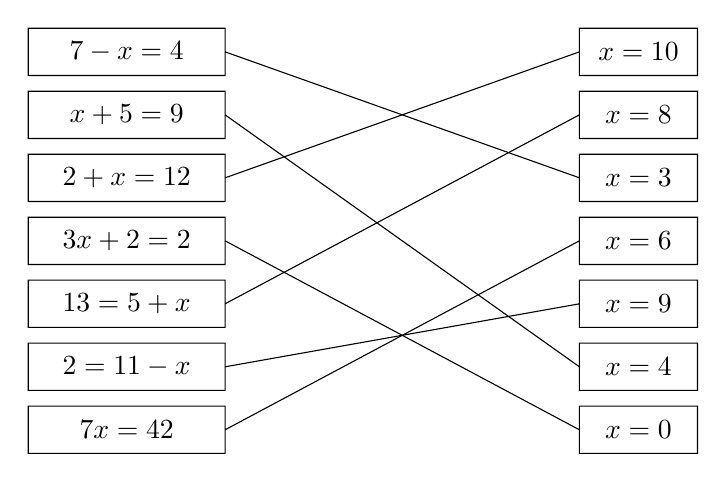
\begin{tikzpicture}
            \draw (0,3) rectangle ++(2.5,0.6) node[midway]{$7-x=4$} ++(0,-0.3) -- (7,1.7) ++(0,-0.3) rectangle ++(1.5,0.6) node[midway]{$x=3$};
            \draw (0,2.2) rectangle ++(2.5,0.6) node[midway]{$x+5=9$} ++(0,-0.3) -- (7,-0.7) ++(0,-0.3) rectangle ++(1.5,0.6) node[midway]{$x=4$};
            \draw (0,1.4) rectangle ++(2.5,0.6) node[midway]{$2+x=12$} ++(0,-0.3) -- (7,3.3) ++(0,-0.3) rectangle ++(1.5,0.6) node[midway]{$x=10$};
            \draw (0,0.6) rectangle ++(2.5,0.6) node[midway]{$3x+2=2$} ++(0,-0.3) -- (7,-1.5) ++(0,-0.3) rectangle ++(1.5,0.6) node[midway]{$x=0$};
            \draw (0,-0.2) rectangle ++(2.5,0.6) node[midway]{$13=5+x$} ++(0,-0.3) -- (7,2.5) ++(0,-0.3) rectangle ++(1.5,0.6) node[midway]{$x=8$};
            \draw (0,-1) rectangle ++(2.5,0.6) node[midway]{$2=11-x$} ++(0,-0.3) -- (7,0.1) ++(0,-0.3) rectangle ++(1.5,0.6) node[midway]{$x=9$};
            \draw (0,-1.8) rectangle ++(2.5,0.6) node[midway]{$7x=42$} ++(0,-0.3) -- (7,0.9) ++(0,-0.3) rectangle ++(1.5,0.6) node[midway]{$x=6$};
        \end{tikzpicture}
    \end{center}

    \newcommand{\red}[1]{\textcolor{rouge}{#1}}
    \begin{minipage}[t]{0.5\linewidth}
        \exercice Soit $x$ la quantité recherchée.
        \begin{align*}
            x+\frac{x}{7} &= 19 \\
            \red{7} \left( x + \frac{x}{7} \right) &= \red{7} \times 19 \\
            7x + x &= 133 \\
            8x &= 133 \\
            \frac{8x}{8} &= \frac{133}{8} \\
            \Aboxed{x &= \frac{133}{8}}
        \end{align*}
    \end{minipage}
    \begin{minipage}[t]{0.45\linewidth}
        \exercice Soit $x$ la quantité recherchée.
        \begin{align*}
            x + \frac{x}{2} &= 16 \\
            \red{2} \left( x + \frac{x}{2} \right) &= \red{2} \times 16 \\
            2x + x &= 32 \\
            3x &= 32 \\
            \Aboxed{x &= \frac{32}{3}}
        \end{align*}
    \end{minipage}

    \exercice Soit $x$ la quantité recherchée.
    \begin{align*}
        x + \frac{x}{5} &= 21 \\
        \red{5} \left( x + \frac{x}{5} \right) &= 21 \\
        5x + x &= 21 \\ 
        6x &= 21 \\ 
        \Aboxed{x &= \frac{21}{6}}
    \end{align*}

    \clearpage
    \exercice 
    \begin{minipage}{0.45\linewidth}
    Soit la $x$ la longueur de la lance.
        \begin{center}
            \begin{tikzpicture}[scale=1.5]
                \fill[blue!10!white] (-1.5,-0.3) rectangle (2,-3.4);
                \draw (0,0) -- (0,-3);
                \draw (0.5,0) -- (0.5,-3);
                \draw (0,0) arc(180:0:0.25);
                \draw (0,-3) arc(-180:0:0.25);
                \node[opacity=0.0] (tmp) at (0.25,-1.5) {\textsc{Lance}};
                \node[rotate around={90:(tmp.center)}] at (0.25,-1.5) {\textsc{Lance}};
                \draw[Latex-Latex] (-0.2,0.25) -- +(0,-3.5) node[midway,left]{$x$};
                \draw[Latex-Latex] (0.7,-3.25) -- +(0,1.75) node[midway,right]{$\dfrac{x}{2}$};
                \draw[Latex-Latex] (0.7,-1.5) -- +(0,1.2) node[midway,right]{$\dfrac{x}{3}$};
                \draw[Latex-Latex] (0.7,-0.3) -- +(0,0.55) node[midway,right]{9};
            \end{tikzpicture}
        \end{center}
    \end{minipage}
    \begin{minipage}{0.45\linewidth}
    Résolvons l'équation : 
        \begin{align*}
            x &= \frac{x}{2} + \frac{x}{3} + 9 \\
            \red{6}x &= \red{6} \left( \frac{x}{2} + \frac{x}{3} + 9 \right) \\
            6x &= 6\frac{x}{2} + 6\frac{x}{3} + 6 \times 9 \\
            6x &= 3x + 2x + 54 \\
            6x \red{-3x-2x} &= 3x + 2x + 54 \red{-3x-2x} \\ 
            \Aboxed{x &= 54}
        \end{align*}

    Donc la lance mesure 54 paumes.
    \end{minipage}
    
    \exercice Dans une entreprise de 320 personnes, il y a 3 fois plus d'hommes que de femmes. Soit $x$ le nombre de femmes, alors il y a 3 fois plus d'hommes, donc $3x$ hommes.

    \begin{align*}
        \mbox{hommes} + \mbox{femmes} &= 320 \\
        3x + x &= 320 \\
        4x &= 320 \\ 
        x &= \frac{320}{4} \\
        \Aboxed{x &= 80}
    \end{align*}

    Donc il y a 80 femmes et $80 \times 3 = 240$ hommes dans cette entreprise. On pourrait dire qu'il y a un quart de femmes, autrement dit \qty{25}{\%} de femmes dans cette entreprise.

    \exercice
    \begin{minipage}{0.4\linewidth}
        \begin{center}
            \begin{tikzpicture}
                \draw (0,0) rectangle +(1,8);
                \draw[Latex-Latex] (1.2,0) -- +(0,8) node[midway,right]{$x$};
                \draw[Latex-Latex] (-0.2,0) -- +(0,2) node[midway,left]{$\dfrac{x}{4}$};
                \draw[Latex-Latex] (-0.2,2) -- +(0,3.2) node[midway,left]{$\dfrac{2x}{5}$};
                \fill[red] (0,0) rectangle +(1,2);
                \fill[green] (0,2) rectangle +(1,3.2);
                \draw[Latex-Latex] (-0.2,5.2) -- +(0,2.8) node[midway,left]{\qty{378}{\EURO}};
            \end{tikzpicture}
        \end{center}
    \end{minipage}
    \begin{minipage}{0.5\linewidth}
        \begin{align*}
            x &= \frac{x}{4} + \frac{2x}{5} + 378 \\
            \red{20}x &= \red{20 \times} \left(\frac{x}{4} + \frac{2x}{5} + 378\right) \\
            20x &= 20\frac{x}{4} + 20 \times \frac{2x}{5} + 20 \times 378 \\
            20x &= 5x + 8x + 7560 \\
            20x \red{-5x-8x} &= 5x + 8x + 7560 \red{-5x-8x} \\
            7x &= 7560 \\
            x &= \frac{7560}{7} \\ 
            x &= \boxed{1080}
        \end{align*}

    Donc le salaire mensuel de cet individu est de \qty{1080}{\EURO}.
    \end{minipage}

    \clearpage
    \exercice Soit $x$ le nombre de moutons dans le troupeau.
    \begin{align*}
        \frac{x}{3} &= x - 20 \\
        \red{3 \times} \frac{x}{3} &= \red{3} \times \left(x-20\right) \\ 
        x &= 3x - 60 \\
        x \red{-3x} &= 3x - 60 \red{-3x} \\
        -2x &= -60 \\
        x &= \frac{-60}{-2} \\ 
        \Aboxed{x &= 30}
    \end{align*}

    Donc il y a 30 moutons dans le troupeau.

    \exercice Soit $x$ la somme reçue par la première personne.
    \begin{itemize}
        \item Si la deuxième personne reçoit \qty{70}{\EURO} de plus que la première, alors elle reçoit $x+70$.
        \item Si la troisième personne reçoit \emph{le double} de ce que perçoit la première moins \qty{150}{\EURO}, alors elle reçoit $2x-150$.
    \end{itemize}

    \vspace{-1.5em}
    \begin{align*}
        \mbox{première personne} + \mbox{deuxième personne} + \mbox{troisième personne} &= 1900\\ 
        x + (x+70) + (2x-150) &= 1900 \\
        4x -80 &= 1900\\
        4x-80 \red{+80} &= 1900 \red{+80} \\
        4x &= 1980\\
        x &= \frac{1980}{4} \\ 
        \Aboxed{x &= 495}
    \end{align*}

    Donc la première personne a reçu \qty{495}{\EURO}, la deuxième \qty{565}{\EURO} et la troisième \qty{840}{\EURO}.

    \exercice Il faut trouver \emph{3 entiers consécutifs} qui, lorsqu'on les additionne, donne 2006. Soit $x$ le premier (le plus petit) des 3 nombres que l'on recherche.\\ 
    Le nombre qui est après $x$ est $x+1$, et celui encore après est $x+2$.

    \begin{align*}
        x + (x+1) + (x+2) &= 2006 \\
        3x + 3 &= 2006 \\
        3x + 3 \red{-3} &= 2006 \red{-3} \\
        3x &= 2003 \\
        \Aboxed{x &= \frac{2003}{3}}
    \end{align*}

    Or $\frac{2003}{3}$ n'est pas un nombre entier, donc ce que l'énoncé nous demande << trouver 3 entiers consécutifs dont la somme est 2006>> est impossible.

    \exercice Il faut trouver \emph{4 nombres pairs consécutifs} dont la somme vaut 196. Par exemple, \{ 18, 20, 22, 24\} sont des entiers pairs consécutifs, mais leur somme vaut $18+20+22+24=82$. Soit $x$ le premier des 4 nombres que l'on recherche (autrement dit, le plus petit), alors le deuxième sera $x+2$, le troisième $x+4$ et le quatrième $x+6$.

    \begin{align*}
        x + (x+2) + (x+4) + (x+6) &= 196 \\ 
        4x + 12 &= 196 \\
        4x + 12 \red{-12} &= 196 \red{-12} \\
        4x &= 184 \\
        x &= \frac{184}{4}\\ 
        \Aboxed{x &= 46}
    \end{align*}

    Donc les nombres attendus sont \{ 46, 48, 50, 52 \}.

    \exercice Soit $x$ le nombre recherché.

    \begin{align*}
        \frac{3}{4}x + \frac{1}{2} &= 1 \\ 
        \red{4 \times} \left( \frac{3}{4}x + \frac{1}{2} \right) &= \red{4 \times} 1 \\ 
        3x + 2 &= 4 \\ 
        3x + 2 \red{-2} &= 4 \red{-2} \\ 
        3x &= 2 \\ 
        \Aboxed{x &= \frac{2}{3}}
    \end{align*}

    \exercice Soit $c$ le côté du carré.
    \begin{itemize}
        \item "D’après la première, il lui reste 39 hommes" $\longrightarrow c^2 + 39$
        \item "la 2eme manière, en mettant un homme de plus par coté, il lui en manque 50" $\longrightarrow (c+1)^2 - 50$
    \end{itemize}

    D'où l'équation : 
    \begin{align*}
        c^2 + 39 &= (c+1)^2 - 50 \\ 
        c^2 + 39 &= c^2 + 2c + 1 - 50 \\
        c^2 + 39 \red{- c^2} &= c^2 + 2c + 1 - 50  \red{- c^2} \\ 
        39 &= 2c + 1 - 50 \\ 
        2c + 1 - 50 &= 39 \\ 
        2c - 49 &= 39 \\ 
        2c - 49  \red{+49} &= 39  \red{+49} \\ 
        2c &= 88 \\ 
        \Aboxed{c &= 44}
    \end{align*}
    
    \exercice On cherche trois entiers consécutifs tels que leur somme vaut 231. Soit $x$ le plus petit des trois nombres, alors les deux autres sont $x+1$ et $x+2$.

    D'où l'équation : 
    \begin{align*}
        x + x+1 + x+2 &= 231 \\
        3x + 3 &= 231 \\
        3x + 3 \red{-3} &= 231 \red{-3} \\
        3x &= 228 \\ 
        x &= \frac{228}{3} \\
        \Aboxed{x &= 76}
    \end{align*}

    Donc les mesures du triangle sont \qty{76}{\centi\metre}, \qty{77}{\centi\metre} et \qty{78}{\centi\metre}.

    \exercice Soit $x$ l'âge d'Alexis. Béatrice est de 3 ans son aîné, donc l'âge de Béatrice est $x+3$. On sait qu'à eux deux, ils ont 31 ans. D'où l'équation : 

    \begin{align*}
        \mbox{âge d'Alexis} + \mbox{âge de Béatrice} &= 31 \\ 
        x + (x+3) &= 31 \\ 
        2x + 3 &= 31 \\ 
        2x + 3 \red{-3} &= 31 \red{-3} \\ 
        2x &= 28 \\ 
        \Aboxed{x &= 14}
    \end{align*}

    Donc Alexis a 14 ans et Béatrice a 17 ans.

    \exercice Le périmètre d'un rectangle vaut : $2 \times \mbox{longueur} + 2 \times \mbox{largeur}$. Posons $x$ la largeur du terrain. Comme le terrain est \emph{3 fois plus long que large}, la longueur vaut $3x$.

    \begin{align*}
        2 \times \mbox{longueur} + 2 \times \mbox{largeur} &= 176 \\
        2 \times x + 2 \times (3x) &= 176 \\ 
        2x + 6x &= 176 \\ 
        8x &= 176 \\ 
        x &= \frac{176}{8} \\ 
        \Aboxed{x &= 22} 
    \end{align*}

    Donc la largeur du terrain est de \qty{22}{\metre}, et sa longueur $22 \times 3 = \qty{66}{\metre}$.

    \clearpage
    \exercice Soit $x$ le nombre recherché.

    \begin{align*}
        3x + 7 &= 4x - 3 \\ 
        3x + 7 \red{-4x} &= 4x - 3 \red{-4x} \\ 
        -x + 7 &= -3 \\ 
        -x + 7 \red{-7} &= -3\red{-7} \\ 
        -x &= -10 \\ 
        \Aboxed{x &= 10}
    \end{align*}

    Le nombre recherché était 10.

    \exercice Soit $x$ le nombre de cailloux du troisième tas.
    \begin{itemize}
        \item 1er tas : $x+30$
        \item 2ème tas : $x - 6$
        \item 3ème tas : $x$
    \end{itemize}

    \begin{align*}
        x+30 + x-6 + x &= 150 \\ 
        3x +24 &= 150 \\
        3x +24 \red{-24} &= 150 \red{-24} \\ 
        3x &= 126 \\ 
        x &= \frac{126}{3} \\ 
        \Aboxed{x &= 42}
    \end{align*}

    Il y a donc 42 cailloux dans le 3ème tas, 72 dans le 1er tas et 36 dans le 2ème.

    \exercice Soit $x$ la masse du bouchon. Alors la bouteille pèse \qty{100}{\gram} de plus que le bouchon, donc $x+100$. Puisque les deux masses font \qty{110}{\gram}, on a l'équation : 

    \begin{align*}
        x + (x+100) &= 110 \\ 
        2x + 100 &= 110 \\ 
        2x + 100 \red{-100} &= 110 \red{-100} \\ 
        2x &= 10 \\ 
        \Aboxed{x &= 5}
    \end{align*}

    Donc le bouchon pèse \qty{5}{\gram} et la bouteille \qty{105}{\gram}.

    \clearpage
    \exercice Pour équilibrer l'équation-bilan, on va compter le nombre d'atomes de chaque élément chimique dans les réactifs et dans les produits, et vérifier qu'on en a bien le même nombre.

    \begin{center}
        \begin{tabularx}{0.9\linewidth}{l|CcCcCcC|}
            &\multicolumn{3}{|c}{Réactifs} && \multicolumn{3}{c|}{Produits}\\\hline
            & $CH_4$ &+& $x0_2$ & $\longrightarrow$ & $CO_2$ &+& $2H_2 O$ \\\hline\hline
            Carbone & 1 &+& 0 & $\longrightarrow$ & 1 &+& 0 \\\hline
            Hydrogène & 4 &+& 0 & $\longrightarrow$ & 0 &+& 4 \\\hline
            Oxygène & 0 &+& $2x$ & $\longrightarrow$ & 2 &+& 2 \\\hline
        \end{tabularx}
    \end{center}

    On en déduit l'équation $2x=4$, d'où $x=2$.
    
    L'équation-bilan est donc $CH_4 + 2O_2 \longrightarrow CO_2 + 2H_2 O$
    
    \exercice 
    \question 
    \begin{align*}
        8x-2 &= 5x-6  & \mbox{il y a un $5x$ à droite, je veux l'enlever}\\
        8x-2\textcolor{rouge}{~-~5x} &= 5x-6\textcolor{rouge}{~-~5x} & \mbox{pour cela, je retire $5x$ de chaque côté}\\
        3x-2 &= -6  & 8x-5x=3x\\
        3x-2\textcolor{vert}{~+~2} &= -6\textcolor{vert}{~+~2} & \mbox{pour me débarrasser du $-2$ à gauche, j'ajoute $+2$}\\
        3x &= -4 & -6+2=-4 \\
        \dfrac{3x}{3} &= \dfrac{-4}{3} & \mbox{j'ai $3x$, mais je veux juste $x$, je vais donc diviser par 3} \\
        x &= \fbox{$-\dfrac{4}{3}$}
    \end{align*}
    \question 
    \begin{align*}
        7x+2 &= 4x+7  & \mbox{il y a un $4x$ à droite, je veux l'enlever}\\
        7x+2\textcolor{rouge}{~-~4x} &= 4x+7\textcolor{rouge}{~-~4x} & \mbox{pour cela, je retire $4x$ de chaque côté}\\
        3x+2 &= +7  & 7x-4x=3x\\
        3x+2\textcolor{vert}{~-~2} &= +7\textcolor{vert}{~-~2} & \mbox{pour me débarrasser du $+2$ à gauche, j'ajoute $-2$}\\
        3x &= +5 & +7-2=+5 \\
        \dfrac{3x}{3} &= \dfrac{5}{3} & \mbox{j'ai $3x$, mais je veux juste $x$, je vais donc diviser par 3} \\
        x &= \fbox{$\dfrac{5}{3}$}
    \end{align*}

    \clearpage
    \exercice Dans l'énoncé, on a l'équation $3y-6=9y-9$. Résolvons-la.
    \begin{align*}
        3y-6 &= 9y-9  & \mbox{il y a un $9y$ à droite, je veux l'enlever}\\
        3y-6\textcolor{rouge}{~-~9y} &= 9y-9\textcolor{rouge}{~-~9y} & \mbox{pour cela, je retire $9y$ de chaque côté}\\
        -6y-6 &= -9  & 3y-9y=-6y\\
        -6y-6\textcolor{vert}{~+~6} &= -9\textcolor{vert}{~+~6} & \mbox{pour me débarrasser du $-6$ à gauche, j'ajoute $+6$}\\
        -6y &= -3 & -9+6=-3 \\
        \dfrac{-6y}{6} &= \dfrac{-3}{-6} & \mbox{j'ai $-6y$, mais je veux juste $y$, je vais donc diviser par -6} \\
        y &= \dfrac{-3}{-6} = \dfrac{3}{6} = \fbox{$\dfrac{1}{2}$} & \mbox{je simplifie la fraction}
    \end{align*}

    On dit dans l'énoncé qu'une des trois équations a la même solution. On va donc tester les trois équations avec la solution qu'on a trouvé, c'est-à-dire $\frac{1}{2}$ :\\

    (*)~ Pour la première $5t=3$, on va calculer $5t$ avec notre solution et voir si cela donne bien 3 ou non.\\
    En l'occurrence, $5t = 5\times \frac{1}{2} = \frac{5}{2} = 2{,}5$. Ca ne fait donc pas 3.\\

    (*) Pour la deuxième $2t-1=0$, on va calculer $2t+1$ avec notre solution et voir si cela donne 0.\\
    En l'occurrence, $2t-1 = 2 \times \frac{1}{2} - 1 = 1 - 1 = 0$. C'est ce que l'on voulait trouver. Donc pour cette équation, $\frac{1}{2}$ est bien une solution.\\

    (*) Pour la troisième, $3t-4=2$, on va calculer $3t-4$ avec notre solution et voir si cela donne 2.\\
    En l'occurrence, $3t-4 = 3 \times \frac{1}{2} - 4 = \frac{3}{2} - 4 = -2{,}5$. Ca ne fait donc pas 2.
\end{questions}
\end{document}